\documentclass[journal,11pt]{IEEEtran}
\usepackage[T1]{fontenc}
\usepackage{amsmath,amssymb,graphicx,booktabs,url}
\usepackage[hidelinks]{hyperref}
\hyphenation{information classification estimation}
\title{Entropy and Mutual Information in\\Modern Machine Learning:\\Estimation, Interpretation, and Limits}
\author{MD FAHIM MUNTASIR}
\begin{document}
\maketitle
\begin{abstract}
Entropy and mutual information provide a mathematical language for uncertainty, dependence, and representation quality in modern machine learning. Their practical use requires distinguishing population quantities from finite-sample estimates and optimization objectives. This report examines three connected questions: how these quantities are estimated, what they mean for learning, and where their interpretation breaks down. It develops the foundations of entropy and conditional information, compares count-based, nearest-neighbor, and neural estimation, and explains connections to cross-entropy, the information bottleneck, and contrastive learning. A controlled feature-selection case study supplies concrete evidence rather than relying solely on a literature survey. Binary and continuous classification experiments test sampling noise, redundant observations, and nonlinear dependence. Marginal selection repeatedly favors duplicated information, whereas conditional selection recovers distinct sources. Yet the additional information does not improve hard classification accuracy in the specified binary model. In the nonlinear model, MI selection achieves 89.32\% mean test accuracy compared with 59.66\% for correlation. An exact XOR derivation establishes a failure of marginal analysis that persists with perfect estimation. The study concludes that information-theoretic quantities are useful only when their estimator, distributional assumptions, and interpretation match the learning objective.
\end{abstract}
\begin{IEEEkeywords}
Entropy, mutual information estimation, representation learning, information bottleneck, contrastive learning, feature selection.
\end{IEEEkeywords}

\section{Introduction}
Entropy and mutual information appear throughout modern machine learning, from probabilistic prediction to learned representations. Entropy describes uncertainty, while mutual information quantifies dependence between observations, labels, or representations. Their origins in Shannon's communication theory \cite{shannon} provide exact mathematical definitions, but an application to finite datasets introduces estimation error, modeling choices, and optimization constraints.

Three questions organize this report. \emph{Estimation} asks how an unknown information quantity can be recovered from samples. \emph{Interpretation} asks whether a score describes predictive uncertainty, task-relevant dependence, compression, or a training objective. \emph{Limits} asks when the estimator, chosen variables, or evaluation metric makes a conclusion unreliable. These distinctions matter because a high empirical score can reflect genuine dependence, sampling noise, or information that is irrelevant to the intended task.

The theoretical discussion connects entropy and MI to cross-entropy training, neural estimation, information-bottleneck objectives, and contrastive learning. To investigate the topic concretely, a feature-selection case study uses distributions with known structure. Binary observations expose redundancy and finite-sample effects, a continuous model isolates nonlinear dependence, and XOR demonstrates a purely interaction-based relationship. Feature selection provides a concrete setting for examining estimation error, redundancy, and the relationship between information and prediction.

The project combines analytical derivations, literature review, and executed simulations. It does not claim to benchmark deep networks or reproduce the neural estimators discussed in the literature. Instead, it uses inspectable examples to show why mathematical information, estimated information, and predictive performance can differ. The final discussion explains which lessons transfer conceptually to learned representations and which require additional empirical evidence.

\section{Theoretical Background}
\subsection{Entropy and conditional entropy}
For a discrete label $Y$ with probability mass function $p(y)$, Shannon entropy in bits is
\begin{equation}
H(Y)=-\sum_y p(y)\log_2 p(y).
\end{equation}
A balanced binary label has entropy one bit. If the label is certain, its entropy is zero. Conditional entropy averages the remaining uncertainty after an observation:
\begin{equation}
H(Y\mid X)=\sum_x p(x)H(Y\mid X=x).
\end{equation}
These definitions concern average uncertainty. They do not mean that each individual sample carries the same information or that uncertainty must decrease for every observed value.

For a Bernoulli variable with success probability $p$, binary entropy is
\begin{equation}
h_2(p)=-p\log_2p-(1-p)\log_2(1-p),
\end{equation}
with the usual convention that $0\log 0=0$. The curve is symmetric around $p=1/2$ and reaches one bit at that point. Binary entropy will connect the simulated observation noise directly to an exact information value.

\subsection{Mutual information and dependence}
Mutual information has the equivalent forms \cite{cover}
\begin{align}
I(X;Y)&=H(Y)-H(Y\mid X),\\
&=\sum_{x,y}p(x,y)\log_2\frac{p(x,y)}{p(x)p(y)}.
\end{align}
It is symmetric and nonnegative, and it is zero exactly when the variables are independent, under the usual definition of the joint distribution. It detects dependence beyond linear correlation. For a discrete label and any admissible feature, $I(X;Y)\leq H(Y)$. In this project that bound is one bit.

An information value is distribution dependent. A change in class balance, measurement process, or deployment population can change the score even when a variable keeps the same name. MI also does not establish causal influence. A variable may predict the label because it is a consequence of the label, shares a common cause, or leaks information from data processing. The supplementary continuous model deliberately uses a label-dependent proxy as a statistical construction, without giving it a causal interpretation.

Continuous features require care. Their differential entropy differs from discrete entropy and can be negative. For mixed continuous features and discrete labels, the general definition through the Kullback--Leibler divergence remains valid, and $H(Y)-H(Y\mid X)$ remains meaningful. We do not compute a differential entropy by applying a discrete count formula to floating-point observations.

\subsection{Conditional information and feature sets}
For a selected set $S$, conditional mutual information measures additional information from a candidate $X_j$:
\begin{equation}
I(X_j;Y\mid X_S)=H(Y\mid X_S)-H(Y\mid X_S,X_j).
\end{equation}
The chain rule gives
\begin{equation}
I(X_S,X_j;Y)=I(X_S;Y)+I(X_j;Y\mid X_S).
\end{equation}
An exact duplicate can have substantial marginal MI but zero additional information once its original is present. This explains why ranking individual scores differs from selecting a jointly informative subset. Redundancy-aware methods such as minimum-redundancy maximum-relevance address this distinction using tractable approximations \cite{peng}.

The data-processing inequality states that processing an observation cannot increase its population information about the target when the required Markov relationship holds. Thus, if a feature is obtained solely by corrupting another feature with independent noise, it cannot contain more target information than its source. Finite-sample estimates can violate the ordering, so a measured violation should prompt an estimation check rather than a new theoretical claim.

\subsection{Information and prediction loss}
The relationship between information and prediction depends on the loss. With an unrestricted probabilistic predictor, minimum expected logarithmic loss equals conditional entropy. Additional conditional information can therefore reduce optimal log loss. Classification accuracy instead depends only on which class has the largest posterior probability. A posterior may become more or less confident without crossing the decision threshold. In that case uncertainty changes but the hard classification decision does not. This distinction is central to interpreting the binary experiment.

\section{Estimation in Modern Machine Learning}
\subsection{Empirical entropy and mutual information}
When the alphabet is small and discrete, counts provide a direct estimate. For $n$ observations, let $\hat p(y)=n_y/n$ and $\hat p(x,y)=n_{xy}/n$. The plug-in entropy estimator is
\begin{equation}
\widehat H(Y)=-\sum_y\hat p(y)\log_2\hat p(y),
\end{equation}
and empirical MI substitutes the corresponding frequencies into the joint-probability formula. Unobserved outcomes contribute no term. This is simple to reproduce, but omitted rare events and random frequency deviations create finite-sample bias. In particular, independent variables need not have exactly factorized empirical frequencies, so their empirical MI can be positive.

For continuous measurements, arbitrary bins change the estimated quantity and introduce resolution choices. Neighbor-based approaches avoid a fixed histogram. Kraskov, Stogbauer, and Grassberger developed estimators for continuous variables \cite{kraskov}; Ross addressed the mixed discrete--continuous setting \cite{ross}. Neighborhood size controls a bias--variance tradeoff, and performance depends on dimension and local geometry. The continuous case study uses a mixed-data estimator, while the binary study uses exact-alphabet counts.

\subsection{Neural estimation and variational bounds}
MINE \cite{mine} learns a neural statistics function $T_\theta$. With $P=P_{XY}$ and $Q=P_XP_Y$, a population lower bound in bits is
\begin{equation}
I(X;Y)\geq\frac{\mathbb E_P[T_\theta]-\ln\mathbb E_Q[e^{T_\theta}]}{\ln 2}.
\end{equation}
The bound follows from the Donsker--Varadhan representation when the expectations exist. Neural optimization searches a parameterized function class; finite samples also replace both expectations. Consequently, a large empirical objective is not automatically a certified lower bound on the unknown population MI. Approximation, optimization, and sampling errors must be distinguished.

\subsection{Recent evidence and practical selection}
Mielniczuk's 2022 review connects information-theoretic variable selection to conditional dependence \cite{review}. Czyz et al. develop a 2023 benchmark spanning distributions with known MI and varied difficulties \cite{beyond}. MINDE uses diffusion models for estimation \cite{minde}. Lee and Rhee evaluate neural estimators on structured image and text data \cite{benchmark}. InfoNet explores learned estimation without test-time optimization \cite{infonet}; we cite its 2024 preprint. Together, these studies illustrate current approaches to evaluating and estimating mutual information across different data types.

An estimator should match the variable types, dimension, sample size, and purpose. Counts are appropriate for the tiny binary alphabet used here. Neighbor methods suit the supplementary univariate continuous features. Neural methods are relevant to learned representations but introduce a training problem of their own. McAllester and Stratos identify limitations on distribution-free, high-confidence MI lower bounds from finite samples \cite{limits}; their result does not imply that all estimation under explicit structural assumptions is impossible.

\section{Interpretation in Modern Machine Learning}
\subsection{Entropy and probabilistic prediction}
For a classifier $q_\theta(y\mid x)$, expected cross-entropy in bits decomposes as
\begin{align}
\mathcal L_{\rm CE}&=\mathbb E[-\log_2 q_\theta(Y\mid X)]\\
&=H(Y\mid X)+\mathbb E_X D_{\rm KL}\!\left(p(\cdot\mid X)\|q_\theta(\cdot\mid X)\right).
\end{align}
The first term is uncertainty in the data distribution. The second measures mismatch between the true conditional distribution and the predictor. Thus a training loss is not itself an entropy estimate: model error and finite-sample generalization also matter. For a fixed representation, reducing model mismatch need not increase its population MI with the label.

Likewise, low predictive entropy $H(q_\theta(\cdot\mid x))$ means the model assigns concentrated probabilities. It does not prove those probabilities are calibrated or correct. A confidently wrong classifier can have low predictive entropy. These distinctions prevent uncertainty measures from being interpreted as direct guarantees of reliability.

\subsection{Representations and the information bottleneck}
Let $R$ be a representation produced from input $X$ through an encoder $p(r\mid x)$. The information-bottleneck objective \cite{ib} balances retained input information against target relevance:
\begin{equation}
\min_{p(r\mid x)}\ I(X;R)-\beta I(R;Y),\qquad \beta\geq0.
\end{equation}
The first term penalizes retained input information, while the second rewards information about the target. A representation that preserves every nuisance detail may be informative about the input without helping prediction. Conversely, excessive compression can discard label-relevant structure. This is an objective for choosing representations, not a theorem that every neural network follows the same information trajectory during training.

The variable definitions are essential. For continuous deterministic representations, MI with the input can be infinite under nondegenerate conditions. Quantization or encoder noise changes the measured problem. A low-dimensional embedding therefore need not have low MI merely because it contains fewer coordinates.

\subsection{Contrastive learning and information surrogates}
Contrastive predictive coding \cite{cpc} learns from paired observations using a contrastive loss. Under its positive-pair and marginal-negative sampling assumptions, a population InfoNCE bound with $N$ candidates is
\begin{equation}
I(U;V)\geq\log_2N-\mathcal L_{\rm NCE}^{(2)},
\end{equation}
where the loss uses base-two logarithms. Since the loss is nonnegative, the bound cannot exceed $\log_2N$, even when true MI is larger. This ceiling limits the bound, not the information the representations can contain. The meaning of shared information also depends on how the views are formed: shared nuisance details need not support a downstream label.

\subsection{A concrete interpretation test}
Feature selection offers a controlled test of these distinctions. Individual MI asks whether a feature carries target information. Conditional MI asks what it adds after other features are observed. Predictive accuracy asks whether that information changes correct hard decisions. The case study below measures these separately. It uses fixed features rather than learned embeddings, so its conclusions about representation learning are conceptual rather than direct neural-network performance evidence.

\section{Case Study Model}
\subsection{Binary observation model}
Let $Y\sim\operatorname{Bernoulli}(1/2)$ and define independent corruption variables $E_1\sim\operatorname{Bernoulli}(p)$ and $E_2\sim\operatorname{Bernoulli}(q)$, where $q=\min(p+0.1,0.49)$. The informative observations are
\begin{equation}
X_1=Y\oplus E_1,\qquad X_2=Y\oplus E_2.
\end{equation}
Here $\oplus$ denotes XOR. Conditional on $Y$, the two observation noises are independent. We add an exact copy $X_3=X_1$ and a degraded copy $X_4=X_1\oplus E_3$, with independent $E_3\sim\operatorname{Bernoulli}(0.05)$. Sixteen independent balanced binary variables complete the twenty-dimensional feature vector. They are independent of the label and of every source variable.

For the first observation, the symmetric construction gives
\begin{equation}
I(X_1;Y)=1-h_2(p).
\end{equation}
At $p=0.2$, this equals approximately $0.278072$ bits. The exact duplicate has the same information and contributes zero conditional information after its original. The degraded copy has an effective error probability $p+0.05-2p(0.05)$. At $p=0.2$, that error is $0.23$, making the copy less informative than $X_1$ but still potentially more informative marginally than $X_2$, whose error is $0.3$.

All of the first four features are associated with the label, but they represent only two independent observation sources. We therefore evaluate source diversity separately from predictive accuracy. Selecting $X_1$ and $X_3$ retrieves two associated features but only one source. Selecting $X_1$ and $X_2$ retrieves both sources. This grouping follows the known construction rather than an inference from correlations.

\subsection{Bayes accuracy for two unequal observations}
For two binary symmetric observations with $0<p<q<1/2$, the more reliable observation determines the optimal hard decision. If the observations disagree, the posterior odds favor $X_1$ because
\begin{equation}
(1-p)q>p(1-q)\quad\Longleftrightarrow\quad q>p.
\end{equation}
If the observations agree, both support the same decision. Consequently the Bayes classifier using both observations predicts $X_1$ and has accuracy $1-p$, exactly as the Bayes classifier using $X_1$ alone.

Nevertheless, the second observation can alter posterior confidence and has positive conditional MI for nondegenerate parameters. This model deliberately separates the goal of capturing additional information from the goal of changing the most likely class. An accuracy tie between marginal and conditional selection is therefore compatible with the information theory. It is not evidence that the second source carries zero information.

\subsection{Continuous nonlinear model}
Let $Z\sim\mathcal N(0,1)$, and let $c=0.6744897502$ satisfy $P(|Z|>c)=1/2$. Define a clean label $B=\mathbf1\{|Z|>c\}$ and an observed label $Y=B\oplus E$, where $E\sim\operatorname{Bernoulli}(0.1)$ independently. The target remains balanced, and the feature $Z$ has
\begin{equation}
I(Z;Y)=1-h_2(0.1)\approx0.531004\text{ bits}.
\end{equation}
Symmetry gives $\operatorname{Cov}(Z,Y)=0$, even though the magnitude of $Z$ strongly predicts the label. We add a weaker continuous proxy $W=0.3(2Y-1)+N$, where $N\sim\mathcal N(0,1)$ independently, together with eighteen independent normal noise features. The proxy has a population Pearson correlation of $0.3/\sqrt{1.09}\approx0.28735$ with the label. This creates a specific, explainable contrast between linear screening and nonlinear dependence screening.

\section{Case Study Experimental Method}
\subsection{Selectors and classifier}
For the binary model, empirical probabilities come from contingency-table counts. Plug-in MI substitutes these frequencies into the population formula. We compare five fixed procedures. All features uses the complete vector. Marginal MI selects the two highest individual MI estimates. Correlation selects the two largest absolute sample Pearson correlations with the label. Greedy conditional MI starts with an empty set and adds the feature giving the largest empirical joint-information increment at each of two steps. The oracle uses the known indices of $X_1$ and $X_2$.

Ties use stable feature-index order. This matters because exact copies necessarily have equal empirical marginal scores. The chosen convention makes runs reproducible and exposes the duplication problem without allowing arbitrary numerical noise to decide between copies. The oracle is a reference based on construction knowledge, not a method available for an unknown real dataset. It also does not guarantee the highest observed finite-sample accuracy for every fitted classifier.

Every method feeds the same decision tree, with maximum depth four and minimum leaf size ten. The tree's random state follows the trial seed. These fixed settings keep the learning rule consistent across comparisons. We do not tune the classifier on the test set. A tree can express the nonlinear magnitude threshold through two splits, so the supplementary example avoids penalizing a selected nonlinear feature with an inherently linear learner.

\subsection{Configurations and independent evaluation}
The binary experiment crosses $p\in\{0.05,0.2,0.35\}$ with training sizes $n\in\{100,300,1000\}$. Each of the nine configurations has thirty independent repetitions. A fresh test sample of 5,000 observations evaluates each repetition, and methods within that repetition share the training and test observations. The full comparison contains 1,350 fitted classifiers. Seeds are deterministic functions of configuration and trial number, as recorded in the source code.

All feature ranking and conditional calculations use training data only. Test labels enter solely into the final accuracy calculation. The continuous experiment uses thirty repetitions with 500 training observations and 5,000 test observations per repetition. It selects one feature using either MI or correlation, then applies the same tree settings. The MI estimator uses three neighbors and explicitly marks features as continuous. Its output is in nats, so the code divides by $\ln 2$ to report bits.

\subsection{Calibration and reported statistics}
A separate calibration experiment repeats a binary channel with $p=0.2$ at sample sizes 50, 100, 300, 1,000, and 3,000. Each size has 200 independent trials. We estimate the signal MI, the MI of one independent binary feature, and the maximum estimated MI among twenty independent binary features. This final statistic illustrates the effect of searching across candidate variables. It is not an estimate of joint information from all twenty variables.

Accuracy summaries report the mean and sample standard deviation across the thirty trials. Plot error bars show one standard deviation, not confidence intervals and not the uncertainty of an individual prediction. Source recovery records whether a two-feature subset contains $X_2$ and at least one member of the $X_1$ source group. The released stability file additionally reports the average pairwise Jaccard overlap of selected index sets across trials. Jaccard measures selection agreement rather than correctness and can underrate interchangeable duplicates.

\section{Case Study Results and Interpretation}
\subsection{Finite-sample information estimates}
Figure~\ref{fig:cal} compares empirical MI with the known channel value. At $n=50$, the signal estimate averages 0.2804 bits, the single null estimate averages 0.0133 bits, and the maximum of twenty null estimates averages 0.0722 bits. At $n=1000$, the corresponding values are 0.2808, 0.00073, and 0.00369 bits. At $n=3000$, the maximum null estimate is about 0.00116 bits.

\begin{figure}[!t]
\centering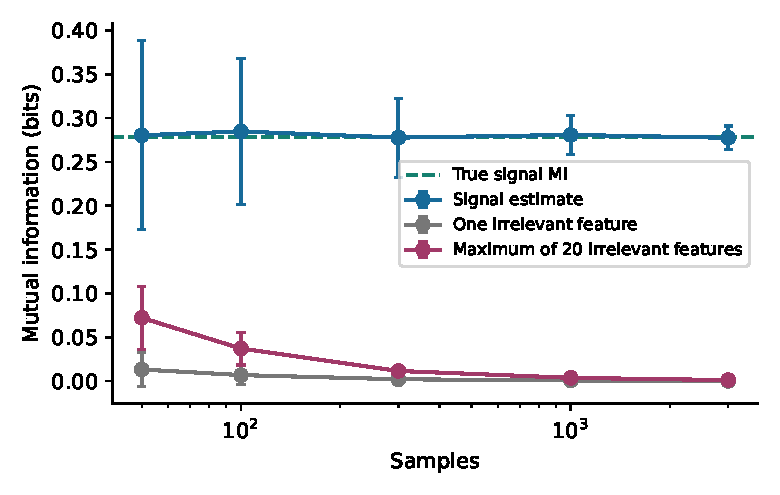
\includegraphics[width=\columnwidth]{figures/estimation.pdf}
\caption{Executed calibration experiment with 200 independent trials per sample size. Error bars indicate one standard deviation. The dashed line is the exact signal value $1-h_2(0.2)$.}\label{fig:cal}
\end{figure}

Positive null values arise because empirical joint frequencies rarely factorize exactly. Nonnegativity of the statistic does not imply genuine dependence. Taking the maximum across twenty candidates increases the apparent null association further. An informative-looking score should therefore be evaluated relative to the sample size and the number of examined variables. The signal estimate need not approach the true value monotonically in a finite set of repetitions, as the reported averages demonstrate.

\subsection{Noise and predictive accuracy}
Figure~\ref{fig:acc} shows the accuracy comparison across all noise levels. Higher corruption lowers attainable accuracy, consistent with the information lost through the observation process. Table~\ref{tab:acc} gives the moderate-noise configuration in detail. At $p=0.2$ and $n=1000$, MI, correlation, conditional MI, and the oracle each average 80.05\% accuracy. The all-feature tree averages 78.48\%.

\begin{figure*}[!t]
\centering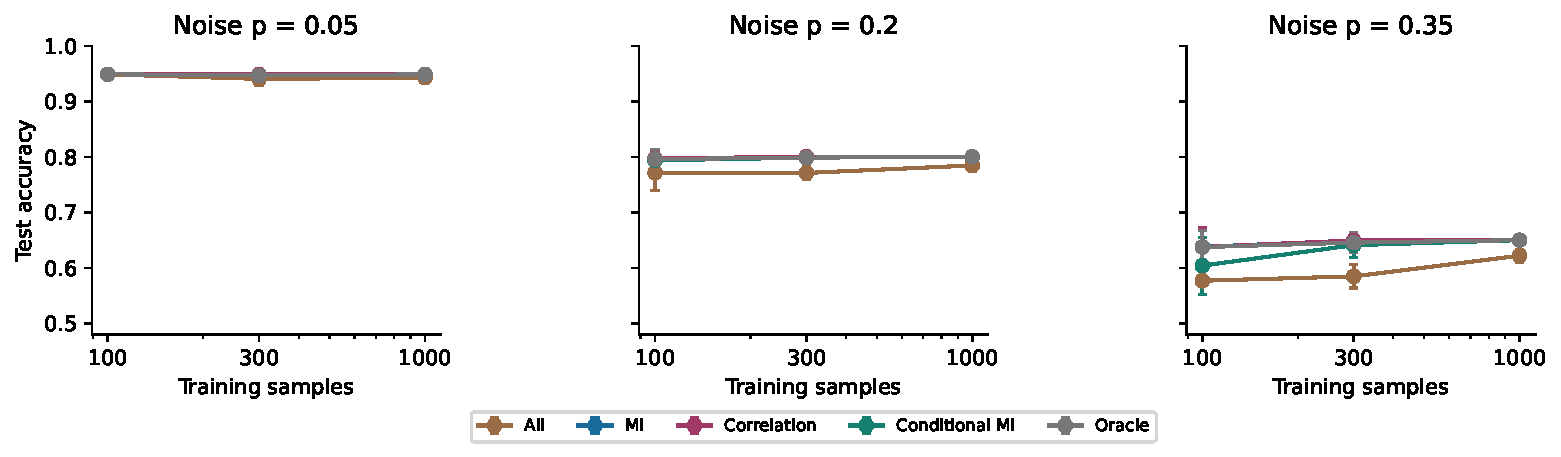
\includegraphics[width=\textwidth]{figures/accuracy.pdf}
\caption{Measured test accuracy over thirty repetitions per configuration. Error bars show one standard deviation across repetitions. All methods use the same fixed tree classifier and shared data within each trial.}\label{fig:acc}
\end{figure*}

\begin{table}[!t]
\caption{Moderate noise $p=0.2$: mean accuracy in percent with standard deviation across thirty trials}
\label{tab:acc}\centering
\begin{tabular}{lrrr}\toprule
Method & $n=100$ & $n=300$ & $n=1000$\\\midrule
All & $77.17\pm3.26$ & $77.12\pm1.11$ & $78.48\pm1.05$\\
MI & $79.74\pm1.26$ & $80.05\pm0.54$ & $80.05\pm0.46$\\
Correlation & $79.74\pm1.26$ & $80.05\pm0.54$ & $80.05\pm0.46$\\
Conditional MI & $79.40\pm1.67$ & $79.89\pm1.01$ & $80.05\pm0.46$\\
Oracle & $79.63\pm1.64$ & $79.89\pm1.01$ & $80.05\pm0.46$\\\bottomrule
\end{tabular}
\end{table}

The all-feature tree has more opportunities to split on irrelevant variables under the fixed settings. This can explain its lower measured accuracy, but other learners or regularization could change the comparison. MI and correlation agree in this balanced binary construction; the continuous experiment tests a separate nonlinear mechanism.

\subsection{Redundancy and source recovery}
At $p=0.2$ and $n=1000$, marginal MI and correlation recover both independent source groups in zero of thirty trials. Conditional MI recovers both in all thirty trials. At $n=100$, conditional MI recovers both in 83.33\% of trials, while each marginal method does so in 3.33\%. The known duplicate construction explains the gap: selecting an original and its exact copy looks optimal to a ranking based on individual relevance.

Despite this source-recovery advantage, conditional MI gives essentially the same classification accuracy. The Bayes derivation predicts precisely this possibility. Two observations provide a more informative posterior, but the less reliable observation cannot overturn the more reliable one when there are only two unequal binary symmetric observations. The experiment therefore separates a successful information objective from a downstream metric that does not reward all additional information.

A natural extension would measure calibrated probabilistic log loss, where posterior confidence matters directly. That experiment was not executed here. We therefore do not infer a measured log-loss improvement from the accuracy results. The exact conditional-entropy relationship explains what an unrestricted optimal predictor could gain, while a fitted decision tree would require separate calibration and evaluation.

\subsection{Nonlinear dependence}
In the continuous model, MI selects the nonlinear feature $Z$ in all thirty repetitions. Correlation selects it in none. The resulting MI pipeline averages 89.32\% accuracy with a 0.75 percentage-point standard deviation. The correlation pipeline averages 59.66\% with a 1.34 percentage-point standard deviation. Figure~\ref{fig:limits} places this result beside source recovery.

\begin{figure*}[!t]
\centering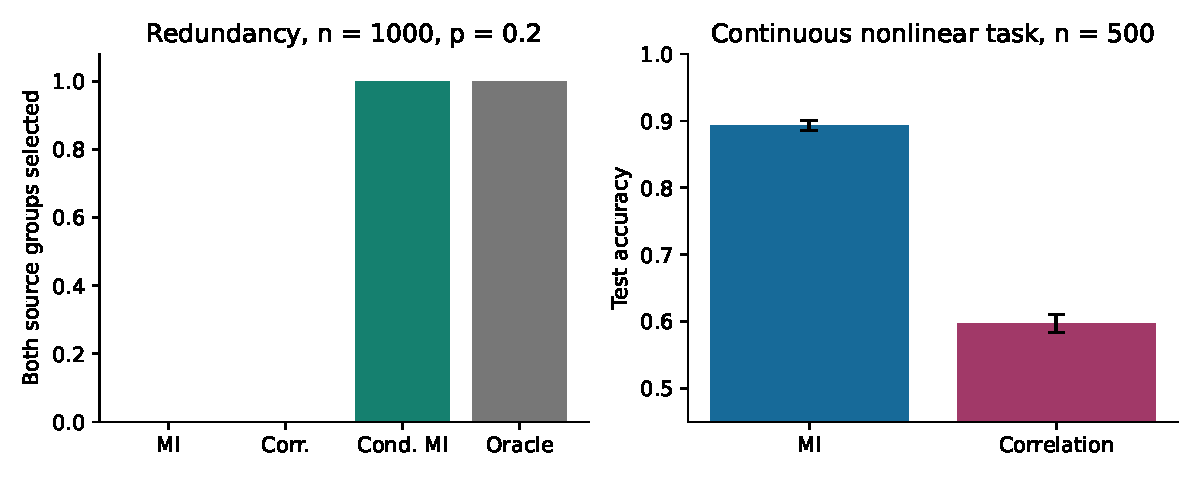
\includegraphics[width=.85\textwidth]{figures/limits.pdf}
\caption{Left: source diversity in the binary model at $p=0.2$ and $n=1000$. Right: mean classification accuracy in the separate continuous nonlinear model. Error bars on accuracy show one standard deviation.}\label{fig:limits}
\end{figure*}

The result agrees with the model: population linear correlation with $Z$ is zero, but the threshold on its magnitude predicts the clean label. With ten-percent independent label corruption, the Bayes accuracy given $Z$ is 90\%. The observed tree accuracy falls slightly below this reference because it estimates thresholds from finite data. This is a demonstration of a known nonlinear mechanism, not evidence that MI selection dominates correlation on every real dataset.

\section{Limits and Open Problems}
\subsection{An XOR counterexample}
Let $A$ and $B$ be independent balanced binary variables and set $Y=A\oplus B$. Given either input alone, the label remains balanced, so
\begin{equation}
I(A;Y)=I(B;Y)=0.
\end{equation}
Given both inputs, the label is deterministic, which gives
\begin{equation}
I((A,B);Y)=1,\qquad I(B;Y\mid A)=1.
\end{equation}
Thus marginal MI can miss jointly decisive variables even with exact population probabilities. More data cannot repair an objective that ignores the needed interaction. The same case challenges greedy conditional selection: before any useful input enters the set, every individual score is zero. With many irrelevant features, the first step may select an irrelevant variable and never reveal the XOR pair. Conditional selection is therefore an improvement for some redundancy structures, not a universal solution to interaction discovery.

\subsection{Estimation and model assumptions}
The plug-in conditional estimator becomes fragile as the selected set grows because the number of joint configurations grows exponentially. A subset of $k$ binary features has up to $2^k$ states before accounting for the label. Our choice of two selected features keeps this manageable and is part of the method's validity boundary. Extending the same counting procedure to hundreds of features would create a different estimation problem.

The continuous estimator also depends on a neighborhood parameter and the geometry of the feature space. This project fixes three neighbors and examines univariate relevance. It does not compare neighborhood choices, neural estimators, or high-dimensional joint estimates. Recent benchmarks emphasize distributional diversity and structured data \cite{beyond,benchmark}; these are appropriate next steps when moving beyond a course-scale example.

The calibration illustrates selection bias across twenty candidates but does not supply a corrected significance test. A practical extension could shuffle labels within the training set, estimate a null distribution for the maximum score, and control feature inclusion at a chosen error level. Such a procedure must repeat all selection steps within the resampling scheme. Comparing a selected maximum to the null distribution for one predetermined feature would underestimate the effect of searching.

\subsection{Generalization and useful information}
All generated test samples follow the same distribution as their training samples. A feature can have high training-distribution MI yet fail under a shift in measurement conditions or class prevalence. Future work could corrupt a proxy differently at deployment or remove a spurious association and measure the resulting accuracy change. This would test robustness beyond independent sampling from a fixed distribution.

Information scores also treat all statistical associations alike. Privacy-sensitive variables, expensive sensors, or post-outcome records may be predictive while unsuitable for deployment. A useful selection objective may need constraints on acquisition cost, availability, fairness, or causal timing. Those constraints cannot be inferred from MI alone. They require a model of how the data will be collected and used.

\subsection{Estimation quality versus optimization usefulness}
A biased information surrogate may still train useful representations, while a more accurate estimate may be costly or have unstable gradients. Evaluating both numerical estimation quality and downstream usefulness is therefore an open methodological problem. Benchmarks with known information values expose failure mechanisms, while realistic image and text data test their practical importance. Our study does not settle whether any neural estimator performs reliably on a given high-dimensional embedding.

\section{Reproducibility}
The accompanying Python script generates all datasets, runs the comparisons, and writes trial-level CSV files and figures. Selected indices allow inspection of redundancy and source recovery. The environment file records package versions. Regeneration requires NumPy, SciPy, pandas, scikit-learn, and Matplotlib; it needs neither an external dataset nor a GPU. Deterministic seeds are recorded in the code. Exact floating-point outputs can depend on the platform and package versions. The numerical results reported here come from the accompanying Python experiments. Neural estimation, information bottleneck methods, and contrastive learning are examined through theoretical analysis and prior literature.

\section{Conclusion}
Entropy and mutual information connect uncertainty, dependence, and representation objectives in modern machine learning. Their use rests on three distinctions. Estimation requires matching a method to data types, sample size, and dimension. Interpretation requires specifying whether a quantity describes label uncertainty, dependence, compression, or an optimization surrogate. Limits arise from finite samples, interaction structure, distribution shift, and the mismatch between information objectives and prediction metrics.

The controlled case study makes these issues concrete. Empirical MI is positive for independent variables in finite samples, and searching many candidates increases apparent null association. Conditional selection recovers distinct sources that marginal ranking duplicates, yet additional information leaves Bayes accuracy unchanged in the specified binary model. In the nonlinear experiment, MI selection achieves 89.32\% rather than 59.66\% mean accuracy. XOR establishes a failure of marginal analysis even with perfect estimation.

These findings support a careful use of information theory across machine learning: define the variables and distribution, distinguish theoretical quantities from fitted objectives, protect evaluation data from selection, and assess the downstream task separately. More information, a larger estimated bound, and better practical predictions are related goals whose agreement must be demonstrated rather than assumed.


\begin{thebibliography}{14}
\bibitem{shannon} C. E. Shannon, ``A mathematical theory of communication,'' \emph{Bell System Technical Journal}, vol. 27, pp. 379--423 and 623--656, 1948, doi: 10.1002/j.1538-7305.1948.tb01338.x.
\bibitem{cover} T. M. Cover and J. A. Thomas, \emph{Elements of Information Theory}, 2nd ed. Wiley, 2006, doi: 10.1002/047174882X.
\bibitem{peng} H. Peng, F. Long, and C. Ding, ``Feature selection based on mutual information: Criteria of max-dependency, max-relevance, and min-redundancy,'' \emph{IEEE Trans. Pattern Anal. Mach. Intell.}, vol. 27, no. 8, pp. 1226--1238, 2005, doi: 10.1109/TPAMI.2005.159.
\bibitem{kraskov} A. Kraskov, H. Stogbauer, and P. Grassberger, ``Estimating mutual information,'' \emph{Phys. Rev. E}, vol. 69, 066138, 2004, doi: 10.1103/PhysRevE.69.066138.
\bibitem{ross} B. C. Ross, ``Mutual information between discrete and continuous data sets,'' \emph{PLOS ONE}, vol. 9, no. 2, e87357, 2014, doi: 10.1371/journal.pone.0087357.
\bibitem{mine} M. I. Belghazi et al., ``Mutual information neural estimation,'' in \emph{Proc. ICML}, PMLR, vol. 80, pp. 531--540, 2018. [Online]. Available: \url{https://proceedings.mlr.press/v80/belghazi18a.html}
\bibitem{review} J. Mielniczuk, ``Information theoretic methods for variable selection---A review,'' \emph{Entropy}, vol. 24, no. 8, 1079, 2022, doi: 10.3390/e24081079.
\bibitem{beyond} P. Czyz, F. Grabowski, J. E. Vogt, N. Beerenwinkel, and A. Marx, ``Beyond normal: On the evaluation of mutual information estimators,'' in \emph{Advances in Neural Information Processing Systems}, vol. 36, 2023. [Online]. Available: \url{https://arxiv.org/abs/2306.11078}
\bibitem{minde} G. Franzese, M. Bounoua, and P. Michiardi, ``MINDE: Mutual information neural diffusion estimation,'' in \emph{Proc. ICLR}, 2024. [Online]. Available: \url{https://openreview.net/forum?id=0kWd8SJq8d}
\bibitem{benchmark} K. Lee and W. Rhee, ``A benchmark suite for evaluating neural mutual information estimators on unstructured datasets,'' in \emph{Advances in Neural Information Processing Systems}, vol. 37, 2024, doi: 10.52202/079017-1472.
\bibitem{infonet} Z. Hu, S. Kang, Q. Zeng, K. Huang, and Y. Yang, ``InfoNet: Neural estimation of mutual information without test-time optimization,'' \emph{arXiv preprint arXiv:2402.10158}, 2024. [Online]. Available: \url{https://arxiv.org/abs/2402.10158}
\bibitem{limits} D. McAllester and K. Stratos, ``Formal limitations on the measurement of mutual information,'' in \emph{Proc. AISTATS}, PMLR, vol. 108, pp. 875--884, 2020. [Online]. Available: \url{https://proceedings.mlr.press/v108/mcallester20a.html}
\bibitem{ib} N. Tishby, F. C. Pereira, and W. Bialek, ``The information bottleneck method,'' manuscript dated 1999, \emph{arXiv:physics/0004057}, 2000. [Online]. Available: \url{https://arxiv.org/abs/physics/0004057}
\bibitem{cpc} A. van den Oord, Y. Li, and O. Vinyals, ``Representation learning with contrastive predictive coding,'' \emph{arXiv preprint arXiv:1807.03748}, 2018. [Online]. Available: \url{https://arxiv.org/abs/1807.03748}
\end{thebibliography}
\end{document}
